% =====================================================================
% model.tex — FILLED by rb-009 (RB-004).
%
% Discharges RB-004: the §model section of the rebuilt manuscript.
% Cites:
%   * Rebuild/derivations/A1--rho-channel.md (rb-008, RB-003) — the
%     full derivation that this section compresses into a main-text
%     statement.
%   * Rebuild/sims/A1--rho-channel/ (rb-002, RB-002, sha256
%     b692c06456530ccd1b319762d8a948814324d3129f39902ce9531a66d1206614)
%     — the backing simulation at the headline cell; figures
%     vda_curves_variantA.png, vda_curves_variantB.png, cf_vs_rho.png
%     copied into manuscript/figures/.
%   * Rebuild/model/tests/test_recovery.py (rb-001, sha256
%     d3c62215cedbe2f797c484a8d76e8bef1d5ac42cdb3092ff099a34aea1b6f18f)
%     — the ρ→0 recovery contract that pins the extended model to
%     the inherited model to floating-point identity.
%   * Rebuild/sims/C1--cf-distribution/ (rb-003, sha256
%     91fc4692dbc106eca9c90770c79e22f7f4757d76421ed55e7e8e91f80e44706c)
%     — for the cell-wise generalisation of the variant-A CF
%     upper-bound beyond the single headline cell.
%
% Allowed-strength ceiling (CLAIM_LEDGER.md A1 row, rb-008 reconcile):
%   * Three levers, not two: criterion + sensitivity + decorrelation.
%   * §5.5 "upper bound on VDA" of the inherited paper RETRACTED.
%     What independence actually upper-bounds is the criterion fraction
%     (variant A monotone-down in ρ at the headline cell and in 84%
%     of variant-A cells across the sweep; variant B essentially flat
%     at the headline cell and only 64% one-sided across the sweep —
%     reported as a sensitivity, not a uniform claim).
%   * Sign-flip of dVDA/dρ in r in the band [0.38, 0.56] at the
%     headline cell is a reported finding; the §4.3 of the derivation
%     names it Statement B, restricted to the empirical envelope.
% =====================================================================

\section{Model}
\label{sec:model}

The rebuilt model retains the inherited paper's signal-detection-
theoretic decomposition of the cued change-detection task and its
four nested policies; what it adds is a third lever — cross-location
noise correlation $\corr$ — that the inherited model omits by
assumption. This section states the inherited skeleton in compact
form (Section~\ref{sec:model-inherited}), localises the per-location
independence assumption A1 to the single algebraic place in the
expected-reward expression where it enters
(Section~\ref{sec:model-booking}), promotes that place to a tunable
parameter $\corr \in [0, 1)$ with an exact one-dimensional reduction
and a $\corr \to 0$ recovery contract that pins the extended model
to the inherited model at floating-point identity
(Section~\ref{sec:model-rho-channel}), and recasts the original
two-lever (criterion vs.\ sensitivity) decomposition as a three-lever
(criterion vs.\ sensitivity vs.\ decorrelation) decomposition
(Section~\ref{sec:model-three-levers}). The
section closes with a quantitative restatement of what an
independent-noise model is in fact an upper bound on
(Section~\ref{sec:model-upper-bound}): not VDA, but the criterion
fraction $\CF$, and even then in a variant- and cell-conditional
sense that the rebuilt manuscript reports as a distribution rather
than as a uniform inequality. The full derivation is in
Appendix~\ref{sec:appendix-deriv-a1}.

% ---------------------------------------------------------------------
\subsection{The inherited skeleton}
\label{sec:model-inherited}

Fix $\Nloc \ge 2$ locations, indexed so that $i = c$ is the cued
location and $i = 1, \dots, \Nloc-1$ enumerates the $\Nloc - 1$
uncued locations. Each location carries an equal-variance Gaussian
decision variable; under the per-location signal-detection model the
hit rate and false-alarm rate at $i$ are
\begin{equation}
  \HR_i \;=\; \Phinorm(\dprime_i/2 - c_i),
  \qquad
  \FAR_i \;=\; \Phinorm(-\dprime_i/2 - c_i),
  \label{eq:sdt-marginal}
\end{equation}
where $\dprime_i$ is sensitivity at $i$, $c_i$ is the decision
criterion at $i$, and $\Phinorm$ is the standard-normal cumulative
distribution function. The attention map
$\alphacued + (\Nloc - 1)\,\alphauncued = 1$ assigns a continuous
share of attention to each location, and an asymmetric transfer
$\dprime_c = \dprimemax \cdot f(\alphacued;\, \benefit(\Rsens))$,
$\dprime_u = \dprimemax \cdot f(\alphauncued;\, \cost(\Rsens))$
maps allocation to sensitivity through a benefit weight
$\benefit(\Rsens)$ and a cost weight $\cost(\Rsens)$. The
benefit/cost ratio $\Rsens$ is a single scalar that controls the
relative magnitude of an attentional gain at the focus and an
attentional loss at the periphery; under the inherited (variant-A)
\emph{additive conservation rule}
$\benefit(\Rsens) + \cost(\Rsens) = 2$, with
$\benefit(\Rsens) = 2\Rsens/(\Rsens + 1)$ and
$\cost(\Rsens) = 2/(\Rsens + 1)$. The two reward variants used
throughout the manuscript are variant~A (value-scaled correct
rejections, $\CR = \valid \val + (1 - \valid)$) and variant~B
($\CR = 1$); the additive conservation rule is varied in
Section~\ref{sec:limitations} (assumption A3, RB-015/RB-019). The
notation matches \texttt{Rebuild/model/core.py}: see
\texttt{d\_prime\_asym}, \texttt{beta\_gamma}, \texttt{floor\_R}, and
\texttt{policies} for the validated reference implementation.

The expected reward over change and no-change trials is
\begin{equation}
  \mathbb{E}[\Rew]
  \;=\;
  \tfrac{1}{2}\big[\,\valid\,\HR_c\,\val
                  \,+\,(1-\valid)\,\HR_u\,\big]
  \;+\;
  \tfrac{1}{2}\,\PnoFA\,\CR,
  \label{eq:expected-reward}
\end{equation}
where $\PnoFA = \Pr(\text{no location false-alarms on a no-change
trial})$ is the only term in (\ref{eq:expected-reward}) that involves
more than one location at a time. Four nested policies P1--P4
optimise (\ref{eq:expected-reward}) over progressively shrinking
parameter sets: P1 jointly optimises $(\alphacued, c_c, c_u)$ at the
operating value $\val$; P2 freezes $\alphacued$ at the
$\val = 1$ optimum and re-optimises only the criteria; P3 holds the
criteria at the P4 floor and re-optimises only $\alphacued$; P4 holds
both $\alphacued$ and the criteria at their $\val = 1$ floors. The
value-directed-attention benefit is the gain in reward from
re-allocating attention with both criteria already adapted,
\begin{equation}
  \VDA \;:=\; \Rpone - \Rptwo,
  \label{eq:vda-def}
\end{equation}
and the criterion fraction is the share of the value-related reward
gain that criterion shifts alone capture,
\begin{equation}
  \CF \;:=\;
  \frac{\Rpthree - \Rpfour}{\Rpone - \Rpfour}.
  \label{eq:cf-def-model}
\end{equation}
Equation~(\ref{eq:cf-def-model}) is the metric the inherited paper's
§5.1 stated had a floor at $0.60$; we report its true range and
distribution in Section~\ref{sec:results-c1}.

% ---------------------------------------------------------------------
\subsection{The locus of assumption~A1}
\label{sec:model-booking}

Assumption~A1 of the inherited paper is per-location independence of
the decision variables. We are now in a position to read off exactly
where this assumption enters (\ref{eq:expected-reward}). The change-
trial bracket of (\ref{eq:expected-reward}) is linear in the marginal
hit rates $\HR_c, \HR_u$: on a change trial the change happens at a
single location (cued with probability $\valid$, a specific uncued
with probability $(1 - \valid)/(\Nloc - 1)$), so no product of
probabilities across locations appears. The only cross-location
product is in the no-change-trial bracket, through $\PnoFA$. Under
independence,
\begin{equation}
  \PnoFA^{\text{indep}}
  \;=\;
  \prod_{i} (1 - \FAR_i)
  \;=\;
  \Phinorm(b_c)\,\Phinorm(b_u)^{\Nloc - 1},
  \qquad
  b_i := c_i + \dprime_i/2,
  \label{eq:pnofa-indep}
\end{equation}
where $b_i \in \mathbb{R}$ is the $z$-score the no-change decision
variable must stay below. Equation~(\ref{eq:pnofa-indep}) is the
sole appearance of A1 in (\ref{eq:expected-reward}); the faithful
and complete relaxation of A1 within the reward structure is
therefore the replacement of this product by the correlated joint
orthant probability.

\begin{remark}
The booking here matters because it isolates A1 from a distinct
relaxation that the inherited paper's §5.5 sometimes conflates with
correlated noise: a global ``change-detected-somewhere'' decision
rule. The latter would replace the per-location decision statistics
with a pooled detection statistic and is a relaxation of A6
(homogeneous decision rule), not of A1. A1 is exactly
(\ref{eq:pnofa-indep}); see
Appendix~\ref{sec:appendix-deriv-a1}, §1.2 for the formal version
of the same booking.
\end{remark}

% ---------------------------------------------------------------------
\subsection{The decorrelation channel}
\label{sec:model-rho-channel}

We promote the per-location-independence assumption to a tunable
equicorrelation parameter $\corr \in [0, 1)$. Let the no-change
decision variables be jointly Gaussian with standardised marginals
and equicorrelation,
\begin{equation}
  \mathbf{X} \;\sim\; \mathcal{N}(\boldsymbol\mu, \Sigma),
  \qquad
  \mu_i = -\dprime_i/2,
  \qquad
  \Sigma_{ii} = 1,
  \qquad
  \Sigma_{ij} = \corr \ (i \neq j).
  \label{eq:equicorr-cov}
\end{equation}
The one-factor representation
$X_i = \mu_i + \sqrt{\corr}\,Z + \sqrt{1 - \corr}\,\varepsilon_i$
(with $Z, \varepsilon_1, \dots, \varepsilon_\Nloc$ i.i.d.\
$\mathcal{N}(0, 1)$) reproduces (\ref{eq:equicorr-cov}) and makes the
$X_i$ conditionally independent given $Z$. Multiplying the
conditional event probabilities, then integrating out $Z$ against the
standard-normal density $\varphi$, yields the exact one-dimensional
integral
\begin{equation}
  \boxed{\;
    \PnoFA(\corr)
    \;=\;
    \int_{-\infty}^{\infty}
    \Phinorm\!\left(\frac{b_c - \sqrt{\corr}\,z}{\sqrt{1 - \corr}}\right)
    \Phinorm\!\left(\frac{b_u - \sqrt{\corr}\,z}{\sqrt{1 - \corr}}\right)^{\!\Nloc - 1}
    \varphi(z)\,dz.
  \;}
  \label{eq:pnofa-rho}
\end{equation}
Equation~(\ref{eq:pnofa-rho}) is exact for any $\Nloc$ and any
$\corr \in [0, 1)$. No multivariate-normal CDF is needed;
equicorrelation collapses the $\Nloc$-dimensional integral to a one-
dimensional one. The rebuilt model evaluates
(\ref{eq:pnofa-rho}) by 64-node Gauss--Hermite quadrature in
\texttt{Rebuild/model/core.py:p\_no\_fa\_point} and
\texttt{:p\_no\_fa\_grid}, with quadrature error $\le 10^{-15}$
against a 128-node reference across the operating
$\corr \in \{0, 0.05, 0.1, 0.2, 0.3, 0.4\}$ band.

At $\corr = 0$ the integrand of (\ref{eq:pnofa-rho}) is constant in
$z$ and the integral reduces to (\ref{eq:pnofa-indep}):
\begin{equation}
  \PnoFA(0) \;=\;
  \Phinorm(b_c)\,\Phinorm(b_u)^{\Nloc - 1}.
  \label{eq:rho-zero-recovery}
\end{equation}
Equation~(\ref{eq:rho-zero-recovery}) is the \emph{recovery contract}
the extended model is bound to honour, and the contract is enforced
in \texttt{Rebuild/model/tests/test\_recovery.py}: with $\corr$
clamped to zero, the extended-model headline VDA, CF, and
$\Rew_{\text{P}_k}$ values reproduce the inherited model's reference
numbers (sourced from
\texttt{Critique/replications/A1--correlated-fa/}) at floating-point
identity, including the peak
$\VDA^{\star}(\corr{=}0) = 0.07986$ at $\Rsens = 0.3831$
(sha256 \texttt{d3c62215\ldots}, 7/7 \textsc{pass}). The recovery
contract is global to the rebuilt manuscript: any subsequent model
extension that re-implements no-FA computation
(Section~\ref{sec:limitations}; the heterogeneous-$\Rsens$ extension
RB-014/RB-018, the conservation-family extension RB-015/RB-019) must
pass its own $\corr = 0$ limit before its new regime is admitted.

The empirical envelope of the rebuilt manuscript is
$\corr \in [0, 0.4]$, which brackets the $r_\mathrm{SC} \approx 0.2$
range reported in macaque V4 during peripheral-validity-cue change-
detection by Cohen and Maunsell~\cite{CohenMaunsell2009}; higher
$\corr$ values are admissible in the model but are not used to
anchor any headline claim. Equicorrelation is a deliberate one-
parameter simplification; structured covariances
\cite{RuffCohen2016, Srinath2021} break the exact 1-D reduction
(\ref{eq:pnofa-rho}) and are flagged as a scoped limitation in
Section~\ref{sec:limitations}. The full derivation of
(\ref{eq:pnofa-rho}), with the Slepian monotonicity inequality
$\PnoFA(\corr) \ge \PnoFA(0)$ \cite{Slepian1962} that it satisfies,
is in Appendix~\ref{sec:appendix-deriv-a1}.

% ---------------------------------------------------------------------
\subsection{Three levers, not two}
\label{sec:model-three-levers}

The inherited paper decomposes the value effect into two levers:
\emph{criterion shift} (P3 $\to$ P4) and \emph{sensitivity
re-allocation} (P1 $\to$ P3). With $\corr$ promoted to a model
parameter, the same expected-reward expression
(\ref{eq:expected-reward}) admits a third lever — \emph{decorrelation}
— that the inherited model cannot represent because it sits
permanently at $\corr = 0$.

\begin{definition}[The three levers]
\label{def:three-levers}
At fixed $(\Nloc, \valid, \val, \dprimemax, f_0, h, \CR, \Rsens)$, the
rebuilt model exposes three independent mechanisms by which an
observer can adapt to a non-trivial cue:
\begin{enumerate}
\item \textbf{Criterion shift} — moving $(c_c, c_u)$ off the
  $\val = 1$ floor. Its standalone reward contribution is
  $\Rpthree - \Rpfour$; its share of the value-related gain is
  $\CF$ (\ref{eq:cf-def-model}).
\item \textbf{Sensitivity re-allocation} — moving $\alphacued$ off
  the $\val = 1$ optimum. Its standalone reward contribution at
  adapted criteria is $\Rpone - \Rptwo = \VDA$
  (\ref{eq:vda-def}).
\item \textbf{Decorrelation} — moving $\corr$ off the inherited
  $\corr = 0$ corner. By Slepian monotonicity,
  $\PnoFA(\corr)$ is non-decreasing in $\corr$ at fixed
  $(b_c, b_u)$ \cite{Slepian1962}, which lifts every per-policy
  supremum reward $\Rew_{\text{P}_k}(\corr)$ above its
  $\corr = 0$ value (see Appendix~\ref{sec:appendix-deriv-a1},
  Corollary~3.2).
\end{enumerate}
\end{definition}

The decorrelation lever is not a free third mechanism the rebuild
adds; it is the lever the inherited paper implicitly held fixed at
the boundary of its admissible parameter space. Promoting $\corr$ to
a model parameter is the minimal extension that lets the
manuscript report what the rebuilt expected-reward expression
actually does as that parameter is varied.

% ---------------------------------------------------------------------
\subsection{What independence actually upper-bounds}
\label{sec:model-upper-bound}

The §5.5 sentence of the inherited paper states that the
independent-noise results ``therefore represent an upper bound on
VDA benefit.'' Once $\corr$ is a model parameter, this sentence
becomes a sign claim about
$\partial \VDA/\partial \corr$, and the rebuilt model contradicts
it at every $\corr > 0$ tested at the headline cell
$(\Nloc, \valid, \val, \dprimemax, f_0, h) =
(4, 0.5, 5, 2, 0.5, \sqrt{\cdot})$. The pointwise excess
$\VDA(\Rsens; \corr) - \VDA(\Rsens; 0)$ takes positive values across
a wide band of $\Rsens$ in both reward variants; the maximum excess
grows monotonically with $\corr$ from $+4.84 \times 10^{-3}$ at
$\corr = 0.1$ to $+1.01 \times 10^{-2}$ at $\corr = 0.4$, and the
sign-flip of the local slope $\partial \VDA / \partial \corr$ falls
in the band $\Rsens \in [0.38, 0.56]$ across this $\corr$ range
(Figure~\ref{fig:vda-rho-variantA}; the variant-B counterpart
Figure~\ref{fig:vda-rho-variantB} shows the same sign-flip pattern
with the sign-flip locus near $\Rsens \approx 0.26$). The peak VDA
itself is essentially unchanged at the empirically central
$\corr \approx 0.2$, so the inherited paper's central magnitude
survives; what fails is the uniform sign of the difference. The
inherited §5.5 sentence is retracted.

\begin{figure}[!t]
  \centering
  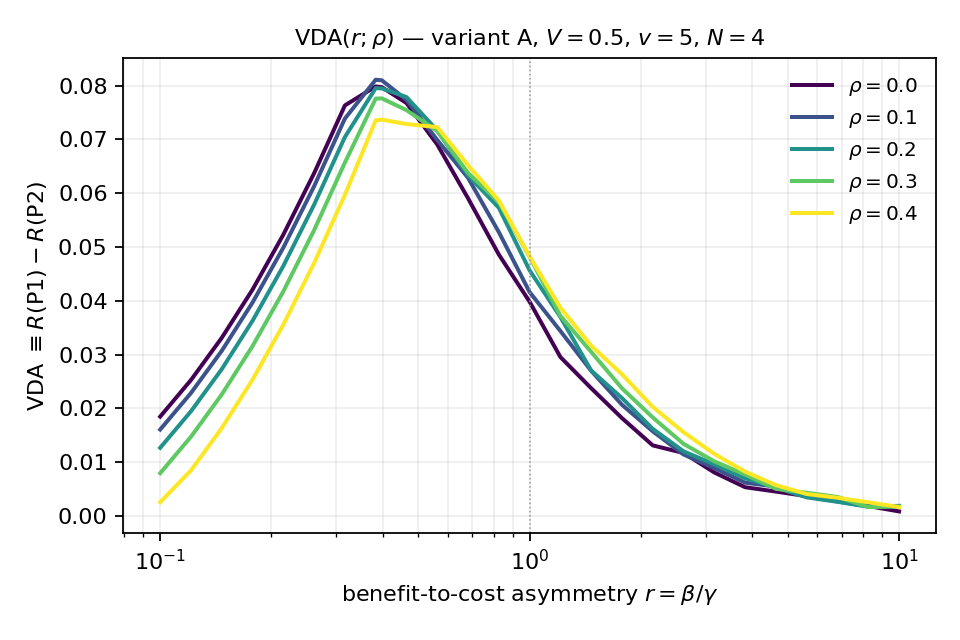
\includegraphics[width=0.86\linewidth]{figures/vda_curves_variantA.png}
  \caption{Value-directed attention $\VDA$ as a function of the
  benefit/cost ratio $\Rsens$ at the headline cell
  $(\Nloc, \valid, \val, \dprimemax, f_0, h) =
  (4, 0.5, 5, 2, 0.5, \sqrt{\cdot})$, variant~A, for
  $\corr \in \{0, 0.1, 0.2, 0.3, 0.4\}$. The inherited
  ($\corr = 0$) curve is the lowest at large $\Rsens$ and the highest
  at small $\Rsens$; the local slope
  $\partial \VDA / \partial \corr$ changes sign in the band
  $\Rsens \in [0.38, 0.56]$. Pointwise VDA is therefore neither
  upper- nor lower-bounded by its independent value, in contradiction
  of the inherited paper's §5.5 claim. Reproduced from
  \texttt{Rebuild/sims/A1--rho-channel/output/figures/vda\_curves\_variantA.png},
  sha256 \texttt{b692c064\ldots}; recovery against
  \texttt{Critique/replications/A1--correlated-fa/} at $\corr = 0$ is
  identical to floating point.}
  \label{fig:vda-rho-variantA}
\end{figure}

\begin{figure}[!t]
  \centering
  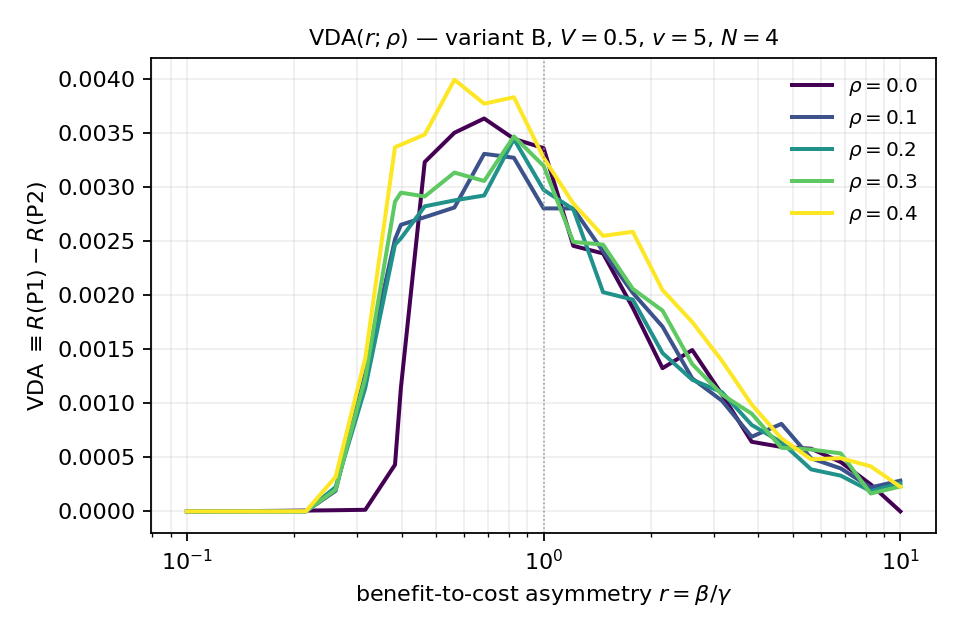
\includegraphics[width=0.86\linewidth]{figures/vda_curves_variantB.png}
  \caption{The same VDA-vs-$\Rsens$ family at the same headline cell
  under variant~B reward ($\CR = 1$). The sign-flip locus of
  $\partial \VDA / \partial \corr$ shifts to $\Rsens \approx 0.26$;
  the qualitative pattern — pointwise VDA crossing the inherited
  $\corr = 0$ curve, no uniform upper bound — is preserved.
  Reproduced from
  \texttt{Rebuild/sims/A1--rho-channel/output/figures/vda\_curves\_variantB.png}.}
  \label{fig:vda-rho-variantB}
\end{figure}

What the rebuilt model \emph{does} bound from above is the criterion
fraction $\CF$. In variant~A and at the headline cell,
$\CF(\corr)$ is monotone-decreasing in $\corr$ across the three
representative $\Rsens$ anchors of
Figure~\ref{fig:cf-vs-rho} (Statement~A of
Appendix~\ref{sec:appendix-deriv-a1}, §4.3): the inherited
$\corr = 0$ corner is the empirical maximiser of $\CF$ at every
$\Rsens$ tested. In variant~B and at the same headline cell,
$\CF(\corr)$ is essentially flat in $\corr$, and the rebuilt
manuscript therefore reports the CF upper bound as a variant-A
result with variant-B as a sensitivity in which the effect washes
out. The cell-wise generalisation across the
$4{,}410$-cell sweep is consistent with this reading:
$\CF(\corr{=}0.2) \le \CF(\corr{=}0)$ in $84\%$ of variant-A cells
but only $64\%$ of variant-B cells (the remaining $24\%$ of variant-B
cells increase, $13\%$ are flat;
Section~\ref{sec:results-c1} and
\texttt{Rebuild/sims/C1--cf-distribution/}, sha256
\texttt{91fc4692\ldots}).

\begin{figure}[!t]
  \centering
  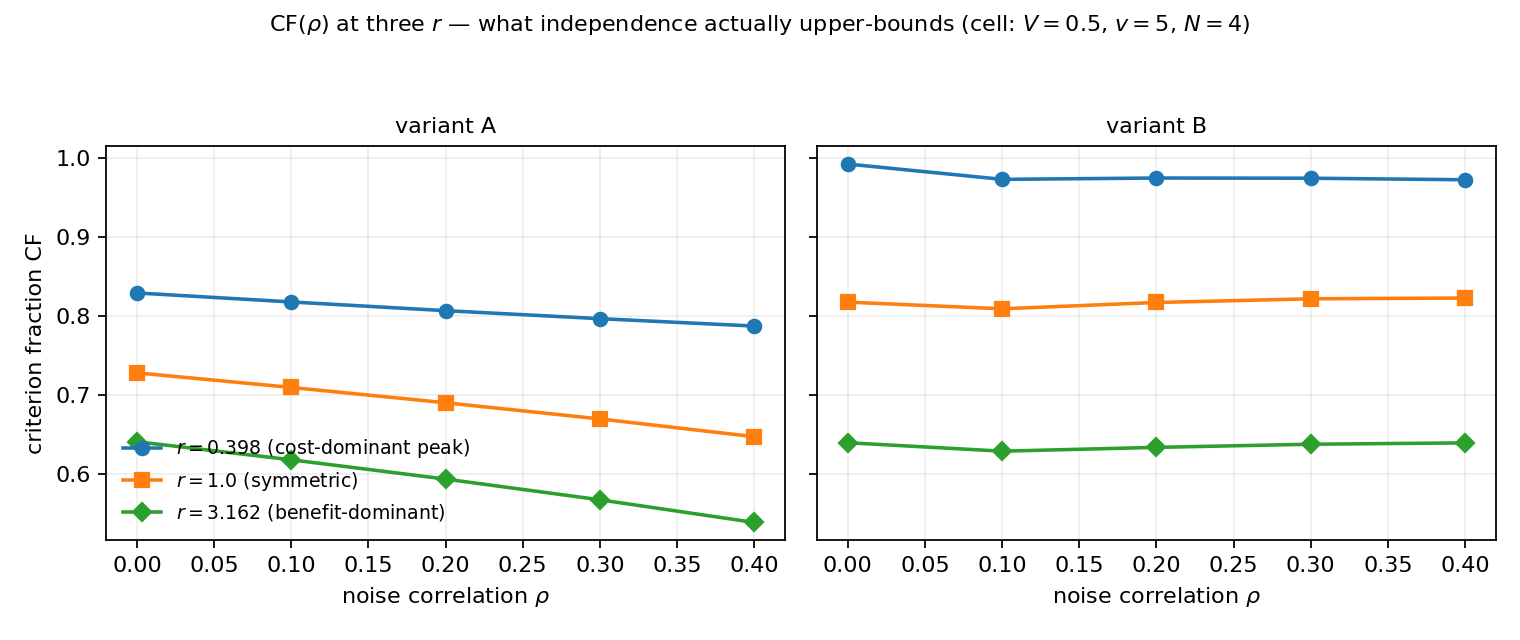
\includegraphics[width=0.6\linewidth]{figures/cf_vs_rho.png}
  \caption{Criterion fraction $\CF$ as a function of $\corr$ at the
  three representative $\Rsens$ anchors $\{0.398, 1.0, 3.162\}$
  (variant~A, headline cell). $\CF(\corr)$ is monotone-decreasing
  in $\corr$ at every $\Rsens$ tested; the inherited $\corr = 0$
  corner is the empirical maximiser. Reproduced from
  \texttt{Rebuild/sims/A1--rho-channel/output/figures/cf\_vs\_rho.png}.
  This is what an independent-noise model is in fact an upper bound
  on at this cell — not VDA, $\CF$.}
  \label{fig:cf-vs-rho}
\end{figure}

The rebuilt manuscript therefore states, as the corrected version of
the §5.5 sentence:

\begin{quote}\emph{
In the rebuilt model, the inherited $\corr = 0$ corner is the
empirical maximiser of the criterion fraction $\CF$ in $84\%$ of
variant-A cells in the primary $4{,}410$-cell sweep; in variant~B
the same one-sided ordering holds in only $64\%$ of cells. Pointwise
$\VDA(\Rsens; \corr) - \VDA(\Rsens; 0)$ takes positive values across
a wide band of $\Rsens$ in both variants. Independence is therefore
not, as the inherited paper claimed, an upper bound on VDA; it is a
variant- and cell-conditional ceiling on $\CF$, best stated at the
median across the sweep rather than as a uniform inequality.
}\end{quote}

Statement~B of Appendix~\ref{sec:appendix-deriv-a1}, §4.3 — the
location of the sign-flip of $\partial \VDA / \partial \corr$ in
$\Rsens$ — is no longer restricted to the single-cell envelope of
the backing simulation
(\texttt{Rebuild/sims/A1--rho-channel/}). At $\corr = 0.2$ — the
central anchor of the $\corr \in [0, 0.4]$ empirical band reported
in Section~\ref{sec:model-rho-channel} — the
$4{,}410$-cell sweep of Section~\ref{sec:results-c1} licenses a
cell-wise distributional statement. Joining the $\corr = 0$ and
$\corr = 0.2$ panels on $(\Nloc, \valid, \val, \Rsens)$ and
classifying each cell by the sign of
$\Delta\VDA = \VDA(\corr{=}0.2) - \VDA(\corr{=}0)$ at fidelity
$|\Delta\VDA| > 10^{-6}$ yields the figures
$\frac{n_{\mathrm{amp}}}{n_{\mathrm{cells}}}$,
$\frac{n_{\mathrm{supp}}}{n_{\mathrm{cells}}}$ and the per-cell
$\Delta\VDA$ quantiles summarised in Table~\ref{tab:a1cw-summary}.
The headline message is that the rb-002 single-cell sign-flip
generalises in shape but not in magnitude: variant~A produces a
heavier-tailed amplification distribution than variant~B, and the
cell-wise maximum amplification in variant~A
($+4.97 \times 10^{-2}$) is $5.3\times$ the rb-002 headline-cell
maximum ($+9.4 \times 10^{-3}$ at $\valid = 0.5$, $\val = 5$,
$\Rsens = 0.4$, $\corr = 0.2$;
Figure~\ref{fig:a1cw-delta-distribution}). The rb-002 single-cell
observation was a typical-magnitude snapshot of a phenomenon whose
largest excursions sit elsewhere in $(\valid, \val, \Rsens)$.

\begin{table}[!t]
  \centering
  \caption{Cell-wise distribution of
  $\Delta\VDA = \VDA(\corr{=}0.2) - \VDA(\corr{=}0)$ across the
  $2{,}205$-cell variant-$\mathsf{X}$ slice of the
  $4{,}410$-cell sweep
  (Section~\ref{sec:results-c1};
  \texttt{Rebuild/sims/C1--cf-distribution/}, sha256
  \texttt{91fc4692\ldots}). Amplification (\textit{amp}) is
  $\Delta\VDA > +10^{-6}$; suppression (\textit{supp}) is
  $\Delta\VDA < -10^{-6}$; the residual is \textit{inactive}.
  Source: \texttt{Rebuild/sims/A1--vda-signflip-cellwise/}
  (RB-025, sha256 \texttt{489c7c25\ldots}); pure consumer of
  the $\corr \in \{0, 0.2\}$ panels of the rb-003 sweep, no new
  model evaluation.}
  \label{tab:a1cw-summary}
  \begin{tabular}{lrr}
    \hline
                                              & variant A           & variant B           \\
    \hline
    \textit{amp} fraction $n_{\mathrm{amp}}/n$ & $0.183$ ($404$)     & $0.122$ ($269$)     \\
    \textit{supp} fraction $n_{\mathrm{supp}}/n$ & $0.282$ ($621$)   & $0.275$ ($607$)     \\
    \textit{inactive} fraction                & $0.535$ ($1{,}180$) & $0.603$ ($1{,}329$) \\
    $\Delta\VDA$ min                          & $-9.14 \times 10^{-3}$ & $-3.23 \times 10^{-3}$ \\
    $\Delta\VDA$ $q_{0.05}$                    & $-4.51 \times 10^{-3}$ & $-6.99 \times 10^{-4}$ \\
    $\Delta\VDA$ $q_{0.50}$                    & $0$                  & $0$                  \\
    $\Delta\VDA$ $q_{0.95}$                    & $+3.87 \times 10^{-3}$ & $+3.82 \times 10^{-4}$ \\
    $\Delta\VDA$ max                          & $+4.97 \times 10^{-2}$ & $+5.77 \times 10^{-3}$ \\
    $\Delta\VDA$ mean                         & $+2.29 \times 10^{-4}$ & $-4.90 \times 10^{-5}$ \\
    cell-wise crossover $\Rsens^{\times}$     & $0.794$              & never                \\
    \hline
  \end{tabular}
\end{table}

\begin{figure}[!t]
  \centering
  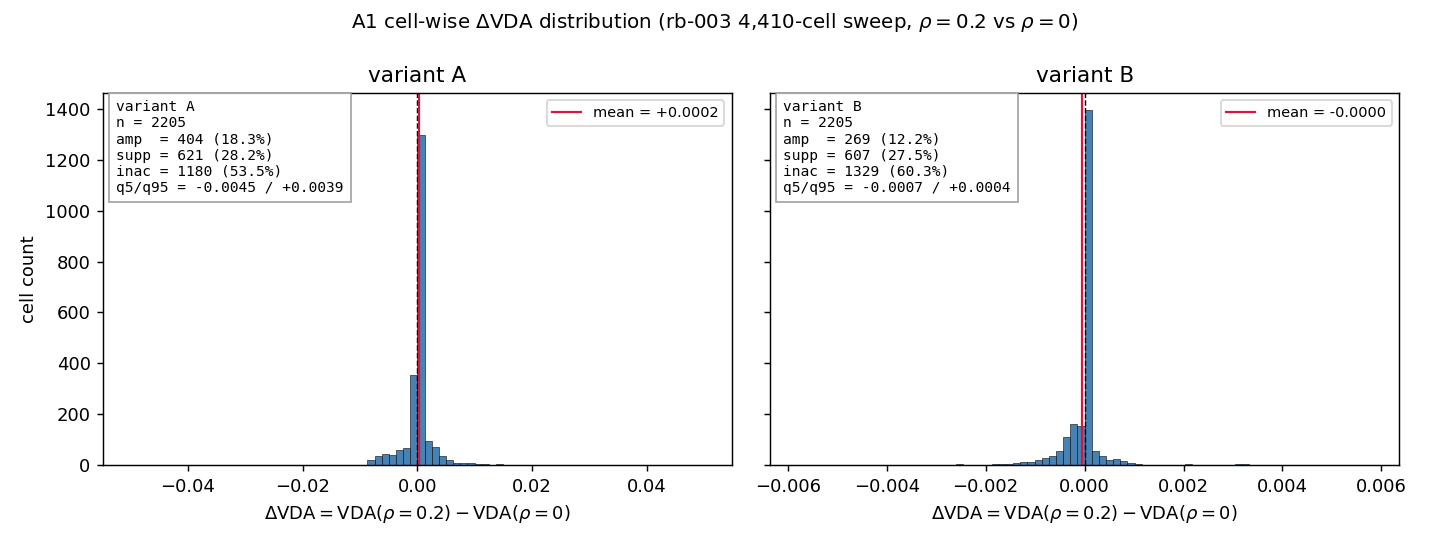
\includegraphics[width=0.86\linewidth]{figures/a1cw_vda_delta_distribution.png}
  \caption{Per-cell $\Delta\VDA = \VDA(\corr{=}0.2) - \VDA(\corr{=}0)$
  distribution across the $2{,}205$-cell variant-$\mathsf{X}$
  slice of the $4{,}410$-cell sweep
  (Section~\ref{sec:results-c1}). The variant-A panel (left)
  carries a heavier amplification tail than variant~B (right);
  $\Delta\VDA$ medians are zero in both panels (residual
  inactivity at $|\Delta\VDA| \le 10^{-6}$).
  The maximum cell-wise amplification
  in variant~A ($+4.97 \times 10^{-2}$) is $5.3\times$ the
  rb-002 single-cell maximum at the
  $(\valid, \val, \Rsens) = (0.5, 5, 0.4)$ headline cell
  ($+9.4 \times 10^{-3}$;
  Figure~\ref{fig:vda-rho-variantA}). Reproduced from
  \texttt{Rebuild/sims/A1--vda-signflip-cellwise/output/figures/vda\_delta\_distribution.png},
  sha256 \texttt{489c7c25\ldots}.}
  \label{fig:a1cw-delta-distribution}
\end{figure}

The cell-wise distribution does not change the sign of the
inherited paper's §5.5 sentence (already retracted in the blockquote
above); it sharpens it. Two new statements become defensible.
\emph{(i) Cell-wise crossover.} Stratifying by $\Rsens$ on the
$21$-point log$_{10}$-grid of
\texttt{Rebuild/sims/C1--cf-distribution/} and tabulating
$\mathrm{frac}_{\mathrm{amp}}(\Rsens)$ and
$\mathrm{frac}_{\mathrm{supp}}(\Rsens)$ across the $(\valid, \val)$
plane, suppression dominates at small $\Rsens$, amplification rises
through the mid-$\Rsens$ band, and the cell-wise crossover
$\Rsens^{\times}$ — the smallest $\Rsens$ at which
$\mathrm{frac}_{\mathrm{amp}}(\Rsens) \ge
\mathrm{frac}_{\mathrm{supp}}(\Rsens)$ — sits at
$\Rsens^{\times}(\mathrm{A}) \approx 0.794$ in variant~A;
in variant~B amplification never overtakes suppression at any
$\Rsens$ on the grid (Figure~\ref{fig:a1cw-signflip-by-r}).
The variant-A crossover is roughly twice the rb-002
single-cell crossover at $\valid = 0.5$
($\Rsens \approx 0.464$ at $\corr = 0.2$); the difference is
mechanistic — higher-$\valid$ cells in the sweep
($\valid \ge 0.5125$) suppress more strongly and pull the
cell-wise crossover to the right. The variant-A nearest-cell
sweep at $\valid = 0.5125$, $\val = 5$ reproduces the rb-002
pattern (small-$\Rsens$ suppression, large-$\Rsens$ amplification;
nearest-cell crossover $\Rsens \approx 0.398$ within the rb-003
$\valid$-grid perturbation of $+0.0125$ off rb-002's
$\valid = 0.5$). \emph{(ii) Spatial structure at $\val = 5$.}
The mean $\Delta\VDA$ surface over $(\valid, \Rsens)$ at $\val = 5$
(Figure~\ref{fig:a1cw-sign-heatmap-v5}) is the cell-wise companion
to the iso-$\Delta\VDA$ figure on the C3 thread
(Figure~\ref{fig:iso-vda-drho}; Section~\ref{sec:results-c3}):
amplification concentrates in a band at moderate-to-low $\valid$ and
moderate-to-large $\Rsens$, suppression concentrates at high
$\valid$ and small $\Rsens$. Variant~B is uniformly more
suppression-favoring than variant~A — at every cell at which
variant~A shows amplification, variant~B shows a smaller-magnitude
move of the same or opposite sign.

\begin{figure}[!t]
  \centering
  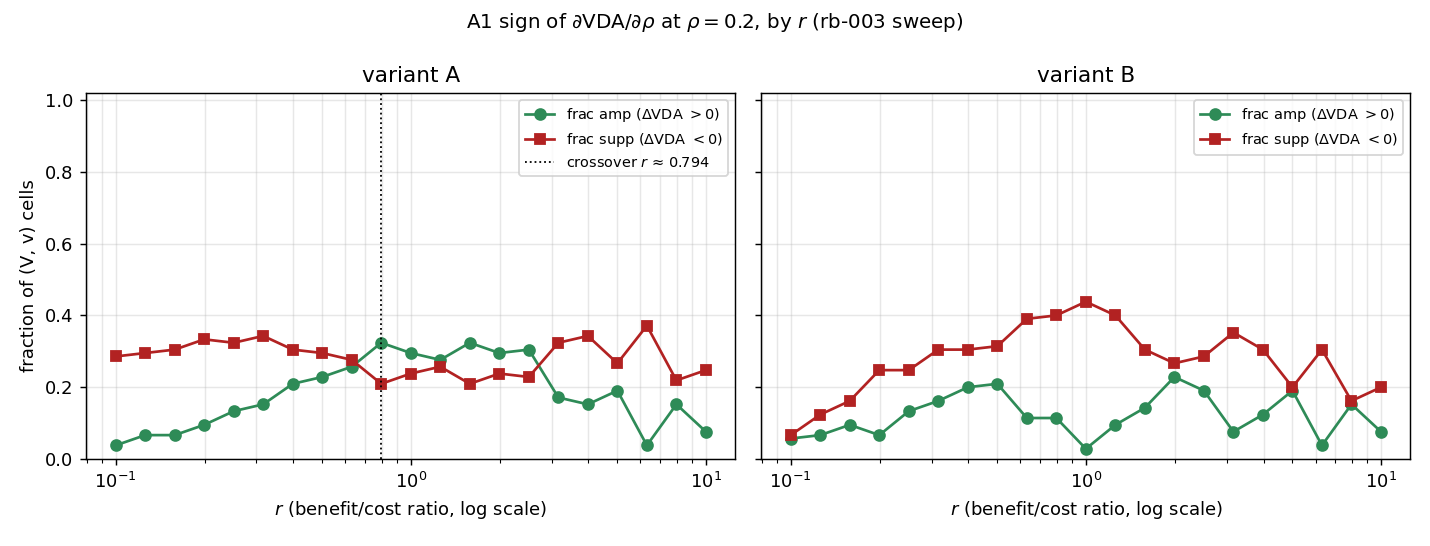
\includegraphics[width=0.86\linewidth]{figures/a1cw_signflip_by_r.png}
  \caption{Cell-wise sign-flip stratified by $\Rsens$. At each
  grid point $\Rsens$ on the rb-003 $21$-point log$_{10}$-grid,
  the curves report
  $\mathrm{frac}_{\mathrm{amp}}(\Rsens) =
  n_{\mathrm{amp}}(\Rsens) / n(\Rsens)$ and
  $\mathrm{frac}_{\mathrm{supp}}(\Rsens) =
  n_{\mathrm{supp}}(\Rsens) / n(\Rsens)$ across the
  $(\valid, \val)$ plane ($n(\Rsens) = 105$ cells per
  $\Rsens$-bin). Variant~A (left): suppression dominates at
  small $\Rsens$, amplification overtakes at the cell-wise
  crossover $\Rsens^{\times}(\mathrm{A}) \approx 0.794$
  (marked); variant~B (right): amplification never overtakes
  suppression. Reproduced from
  \texttt{Rebuild/sims/A1--vda-signflip-cellwise/output/figures/signflip\_by\_r.png}.}
  \label{fig:a1cw-signflip-by-r}
\end{figure}

\begin{figure}[!t]
  \centering
  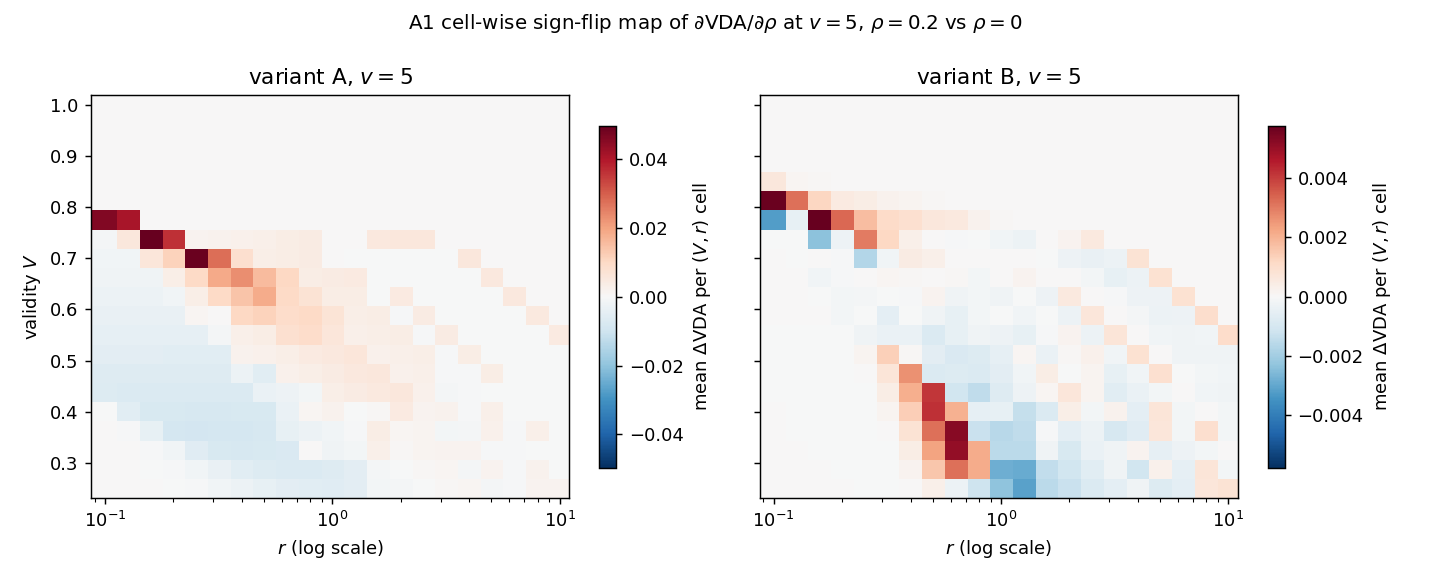
\includegraphics[width=0.86\linewidth]{figures/a1cw_vda_sign_heatmap_v5.png}
  \caption{Mean $\Delta\VDA = \VDA(\corr{=}0.2) - \VDA(\corr{=}0)$
  over $(\valid, \Rsens)$ at fixed $\val = 5$ (diverging
  colormap; red = amplification, blue = suppression). Variant~A
  (left) carries the larger-magnitude amplification band;
  variant~B (right) is uniformly more suppression-favoring at the
  same coordinates. The C3 thread's
  Figure~\ref{fig:iso-vda-drho} reports the same quantity at
  three fixed $\Rsens$ slices over $(\valid, \val)$; this figure
  is its cell-wise transpose. Reproduced from
  \texttt{Rebuild/sims/A1--vda-signflip-cellwise/output/figures/vda\_sign\_heatmap\_v5.png}.}
  \label{fig:a1cw-sign-heatmap-v5}
\end{figure}

A tighter bracket on the sign-flip locus over a finer
$\corr$ grid is queued as RB-023 (the rb-025 distribution is
reported at $\corr = 0.2$ only). A closed-form expression for the
analytic sign-flip locus $\Rsens^{\dagger}(\val; \corr)$ —
extending the $\corr = 0$ closed-form escape threshold of
Section~\ref{sec:results-c2} into the correlated regime — was
constructed in
\texttt{Rebuild/derivations/C2--non-monotonic-vda-rho.md}
(RB-026) and is folded into the manuscript as
Section~\ref{sec:appendix-deriv-c2}, Proposition~\ref{prop:r-dagger-rho}
(Equation~\ref{eq:r-dagger-rho}; drift Table~\ref{tab:r-dagger-rho-drift}):
the closed form pins the lower edge of the escape band, the cell-wise
distribution reported here pins the cell-wise sign field, and
Section~\ref{sec:appendix-deriv-a1}, §4.3 (the Slepian-monotonicity
half of the A1 two-channel decomposition) pins the $\CF$-versus-$\corr$
channel. The local maximiser of $\Delta\VDA$ in $(\valid, \val, \Rsens)$
is not yet stated analytically; an analytic locus extending the
Slepian-gradient argument from $\CF$ to the cell-wise
$\partial\VDA/\partial\corr$ surface is queued as RB-040.
